%\documentclass{article}
%\documentclass[11pt]{article}   % Preset settings for two columns

\documentclass{llncs}

%\setlength{\textheight}{9.0in}
%\setlength{\textwidth}{6.5in}
%\setlength{\columnsep}{0.375in}
%\setlength{\oddsidemargin}{0.0in}
%\setlength{\topmargin}{0.0in}
%\setlength{\headheight}{0.0in}
%\setlength{\headsep}{0.0in}
%\setlength{\parindent}{1pc}

%\usepackage{doublespace}

\usepackage[pagewise]{lineno}       % For line number
\linenumbers

\usepackage{alltt}                         % For program with subscript
\usepackage[mathcal]{euscript}             % For special math symbol

\usepackage{graphicx}                      % For EPS figure
\usepackage{times}                         % For PDF font

%\usepackage{hyperref}                      % For hyper link, should be the last one 

\usepackage[ruled, vlined]{algorithm2e}    % For algorithm, 
                                           % it seems a bug make it has to be here

%\usepackage{psfig}                        % For old PS figure

%\pagestyle{empty}                         % No page Numbering
\pagestyle{plain}                         

%%%% Define theorem
%\newtheorem{theorem}{Theorem}[section]

%------------------------------------------------------------------------- 
%------------------------------------------------------------------------- 

\begin{document}

%--------------------

% title.tex

\date{}      %%%% so that date does not print.

\title{ Structure and algorithm for \\implementing OpenMP workshares}

\author{Guansong Zhang, Raul Silvera, Roch Archambault \thanks{The
    opinions expressed in this paper are those of the authors and not
    necessarily of IBM.}  }

%\thanks{The opinions expressed in this paper are those of the
%  authors and not necessarily of IBM.}


\institute{IBM Toronto Lab \\
Toronto \\
ON, L6G 1C7, Canada}

%\author{Guansong Zhang, Raul Silvera, Roch Archambault\\ 
%\\
%\small IBM Toronto Lab \\ 
%\small Toronto \\ 
%\small ON, L6G 1C7, Canada}


\maketitle

\thispagestyle{empty}

% abstract.tex

\begin{abstract}
  Barrier synchronization is an important and performance critical
  primitive in many parallel programming models, including the popular
  OpenMP model.  In this paper, we compare the performance of several
  software implementations of barrier synchronization and introduce a
  new implementation, \emph{distributed counters with local sensor},
  which considerably reduces overhead on POWER3 and POWER4 SMP
  systems.  Through experiments with the EPCC OpenMP benchmark, we
  demonstrate a 79\% reduction in overhead on a 32-way POWER4 system
  and an 87\% reduction in overhead on a 16-way POWER3 system when
  comparing with a fetch-and-add implementation.  Since these
  improvements are primarily attributed to reduced L2 and L3 cache
  misses, we expect the relative performance of our implementation to
  increase with the number of processors in an SMP and as memory
  latencies lengthen relative to cache latencies.

  \vspace{0.5cm}

  \textbf{Keywords. } barrier, synchronization, multiprocessor,
  distributed counter
\end{abstract}




%--------------------

%\section{Background}

There are many loop transformation techniques existing
today\cite{All02}. And almost all of them can be applied for more than
one kind of code optimizations. For example, loop interchange is
widely used to improve data locality in cache management. Meanwhile it
also can be used to exploit parallelism, such as vectorization, and
even coarse-grained parallelism.  Unfortunately, the transformations
for different optimization purposes do not always work in harmony.

Suppose we have a loop nest, we all know that the loop with stride-one
access of the references should be put to the innermost position to
achieve maximum spatial reuse in cache. So a loop permutation
algorithm will try to calculate such a loop order while keeping the
dependence constrains of the original loop nest.

On the other hand, in an automatic parallelizing compiler, one would
like to parallelize the outermost loop to reduce the parallel region
setup overhead, and leave more code in the inner loop for other
optimization opportunities. For example, in a compiler supporting
OpenMP \cite{Cha01} standard, the straight forward way of generating
parallel code is to parallelize a loop as a parallel do. In this note,
we will concentrate on this kind of \emph{parallelizable} loop only.

Much research has studied different approaches to solve this problem.
A well known technique is \emph{Unimodular transformation}
\cite{Mic91}, a compound loop transformation algorithm aiming at
integrating different loop transformations for a specific goal and
target machine, reducing the problem of finding the best
transformation combination to finding the best unimodular matrix.

Another technique is \emph{Loop selection}\cite{All02}, which
parallelizes all the parallelizable loops, then uses heuristics to
select the next one as sequential, expecting to find more
parallelizable loops after that. It is easier to implement compared to
unimodular transformation.

Our work is based on the idea of loop selection, but different from
the original one in two aspects: a) given our target is an OpenMP node
program, we only need to find one parallelizable loop, avoid
generating code with nested parallelism; b) our heuristics are
directly linked to data locality, unlike the original loop selection
suggested to pick a loop with most ``$<$'' directions to parallelize.





%\section{Summary of Invention} 

In this note, we further improve a loop permutation algorithm to
balance data locality and coarse-grained parallelism in an SMP
environment.

Based on the concept of dependence vectors, we define a multiply
operation in the dependence vector matrix, and prove that under
certain conditions a loop can be permuted to an outer level and still
be parallelizable. Using this condition we add another pass in the
loop selection algorithm for locality to explore coarse-grained
parallelism.

We will see that by carefully choosing the heuristics, we can greatly
improve the performance of an auto-parallelized program. For a typical
test, we reduce more than 50\% execution time on a POWER4 system.



%\newpage

\section{Description}
\label{description}

Before we presenting our discussion in details, we need to introduce
the underlining model to analyze the problem.

\subsection{Analyzing model}
\label{sec:model}

The data dependence vectors\cite{Ban88} are still our principle tools
to analyze and verify the transformation that we are going to apply on
a loop nest. Suppose $\vec{\delta} =\{\delta_{1}\dots\delta_{n}\}$
is a hybrid distance/direction vector with the most precise
information derivable. It represents a \emph{data dependence} between two
array references, corresponding left to right from the outermost loop
to innermost loop enclosing the references. Data dependences are
\emph{loop-independent} if the accesses to the same memory location
occur in the same loop iteration; they are \emph{loop-carried} if the
accesses occur on different loop iterations.

For example, if we have

{\small
\begin{alltt}
 DO i\(\sb{1}\) = 1, U\(\sb{1}\)
   DO i\(\sb{2}\) = 1, U\(\sb{2}\)
     \dots
     DO i\(\sb{n}\) = 1, U\(\sb{n}\)
\(S\sb{1}\)     A(\(f\sb{1}\)(i\(\sb{1}\),\(\dots\),i\(\sb{n}\)),\(\dots\),\(f\sb{m}\)(i\(\sb{1}\),\(\dots\),i\(\sb{n}\)))=\(\cdots\)
\(S\sb{2}\)     \(\cdots\)=A(\(g\sb{1}\)(i\(\sb{1}\),\(\dots\),i\(\sb{n}\)),\(\dots\),\(g\sb{m}\)(i\(\sb{1}\),\(\dots\),i\(\sb{n}\)))
\(T\sb{1}\)     B(\(u\sb{1}\)(i\(\sb{1}\),\(\dots\),i\(\sb{n}\)),\(\dots\),\(u\sb{m}\)(i\(\sb{1}\),\(\dots\),i\(\sb{n}\)))=\(\cdots\)
\(T\sb{2}\)     \(\cdots\)=B(\(v\sb{1}\)(i\(\sb{1}\),\(\dots\),i\(\sb{n}\)),\(\dots\),\(v\sb{m}\)(i\(\sb{1}\),\(\dots\),i\(\sb{n}\)))
     END DO
     \dots
   END DO
 END DO
\end{alltt}
}

as a loop nest from $L_{1}$ to $L_{n}$, we may have two dependences
$\vec{\delta}_{A}$ and $\vec{\delta}_{B}$ characterizing the nested
loops, which were caused by $S\sb{1}$/$S\sb{2}$ and
$T\sb{1}$/$T\sb{2}$. For simplicity, we assume that $f$, $g$, $u$, $v$
are linear functions of the loop induction variables in this note.

Furthermore,

\begin{displaymath}
\left[ 
\begin{array}{c}
\vec{\delta}_{A} \\
\vec{\delta}_{B}
\end{array}
\right]
\end{displaymath}

is a $2 \times n$ \emph{dependence matrix}, denoted as $\mathcal{D}$.
More generally, the number of rows in a dependence matrix may be from
one to any positive number, depending on how many references in the
loop body.

We introduce two theorems.

\begin{theorem}[C-level interchangeable] \label{theorem:interchange}
  Loop $L_{c}$ and $L_{c-1}$ is interchangeable if and only if that
  $\forall \vec{\delta} \in \mathcal{D}$, $\vec{\delta} \neq
  (=^{(c-2)} < > \ldots)$, where ``$=^{(c-2)}$'' means there are
  $(c-2)$ directions as ``$=$'' before the first ``$<$''.
\end{theorem} 

Theorem \ref{theorem:interchange} and its variant forms can be found
in \cite{Zim90} and other literatures. We will not prove it here, and
use it directly for our own theorem later.

\begin{theorem}[P-level parallelizable] \label{theorem:parallelize}
  Loop $L_{p}$ can be parallelized as a parallel do if and only if
  that $\forall \vec{\delta} \in \mathcal{D}$, $\vec{\delta} \neq
  (=^{(p-1)} < \ldots)$.
%, where ``$=^{(p-1)}$'' means there are $(p-1)$
%  directions as ``$=$'' before the first ``$<$''.
\end{theorem} 

The proof for Theorem \ref{theorem:parallelize} is trivial. By the
definition of parallel do, it can not carry any dependence.

Next, we define a \emph{multiply} operation on a dependence vector.

Let $ \vec\sigma=\vec{\sigma}_{a} \times \vec{\sigma}_{b}$, where
$\forall \sigma_{j} \in \vec\sigma, \sigma_{j} = \sigma_{a_{j}} \times
\sigma_{b_{j}}$. The multiplication of the two dependence distance is
defined as following, it is unknown if one of the distance is unknown.
Otherwise it will be the regular multiplication on two integers. If
one of the distance is only a direction, it is treated as 1 or -1, and
after the multiplication, converted back to a direction .

Let $\vec{\sigma}_{p}$ and $\vec{\sigma}_{p-1}$ be the $p^{th}$,
$(p-1)^{th}$ column vector of dependence matrix $\mathcal{D}$, then we
have

\begin{theorem}[Keeping parallelizable] \label{theorem:keep}
  A p-level parallelizable loop $L_{p}$ can be interchanged to
  $L_{p-1}$ and becomes (p-1)-level parallelizable if and only if that
  $\forall \sigma_{j} \in \vec{\sigma}$, where $\vec{\sigma} =
  \vec{\sigma}_{p-1} \times \vec{\sigma}_{p}$, either
  \begin{itemize}
  \item $\sigma_{j}=0$ or 
  \item the $j^{th}$ dependence in $\mathcal{D}$ is not carried by
    $L_{p-1}$
  \end{itemize}
\end{theorem} 

\begin{flushleft}
\textbf{Prof} 
\end{flushleft}

We start from proving the ``\emph{if}'' direction of the theorem.

Suppose $\forall \sigma_{j}=0$. 

Fist we can assert that $L_{p-1}$ and
$L_{p}$ is interchangeable. Otherwise, according to Theorem
\ref{theorem:interchange} there is a dependence vector $\vec{\delta}$
has the form of $(=^{(p-2)} < > \ldots)$. This will conflict with the
fact that all $\sigma_{j}$ is zero.
Second, we prove that the $L_{p}$ will become $(p-1)$-level
parallelizable after interchanging with $L_{p-1}$.  Otherwise, from
Theorem \ref{theorem:parallelize}, there will a dependence vector
$\vec{\delta}$, of the format $(=^{(p-2)} < \ldots)$, in the
dependence matrix preventing it from being parallelized after the
interchange. Considering the format of the $\vec{\delta}$ before the
interchange, given that all $\sigma_{j}$ is zero, it should be in the
form of $(=^{(p-1)} < \ldots)$. This conflicts the fact that $L_{p}$
is parallelizable according to Theorem \ref{theorem:parallelize}.

If $\exists \sigma_{j} \neq 0$, we let $\vec{\delta}$ be the
dependence vector on the $j^{th}$ row of the matrix. It should have
one of the following formats $(\cdots^{(p-2)} < < \ldots)$,
$(\cdots^{(p-2)} < > \ldots)$, $(\cdots^{(p-2)} > < \ldots)$,
$(\cdots^{(p-2)} > > \ldots)$, where $\cdots^{(p-2)}$ is the leading
$(p-2)$ positions. Since $L_{p-1}$ does not carry any dependences as
in the given condition, $\cdots^{(p-2)}$ has be in the format of
$(= \ldots = < \ldots)$, in order for the $\delta$ to be valid. Therefor
$L_{p}$ can be interchanged with $L_{p-1}$ and kept being
parallelizable.

Similarly we can prove the ``\emph{only if}'' direction. It is not
important in our algorithm, we will omit it here.

\begin{flushright}
\textbf{End of Prof} 
\end{flushright}

\begin{theorem}[Outermost parallelizable] \label{theorem:outermost}
  Loop $L_{o}$ can be parallelized at the outermost level if and only
  if that $\vec{\sigma} = \vec{0}$, where $\vec{\sigma}$ is the
  $o^{th}$ column vector of dependence matrix $\mathcal{D}$.
\end{theorem} 

This is a direct conclusion from Theorem \ref{theorem:keep}. It is
actually used in \cite{All02} for loop selection.

%\subsection{Permutation algorithms}
%\label{sec:algorithms}

%Based on our discussion in the previous section, we try to find a
%permutation in favor of both data locality and parallelism.

%{\small
%\begin{algorithm}[h]
%%  \SetLine %this is for setting vertical line with keyword end
%  \SetKw{KwBreak}{break}
%  \SetKwInOut{Input}{Input}
%  \SetKwInOut{Output}{Output}
%  \Input{A desired loop permutation order $O=(L_1,L_2,...,L_n)$, \\
%    the original dependence matrix $\mathcal{D}$ for the loop}
%  \Output{A nearby permutation $P$}
%  \BlankLine

%  \Begin {
%    \If{$\forall \delta \in \mathcal{D}$, $O$ is legal}{
%      \KwRet $O$ \;
%    }
%    $P:=\emptyset$; $k:=0$; $m:=n$\;
%    \While{$O \neq \emptyset$} {
%      \For{$i:=1$ \KwTo $m$} {
%        \If {$\forall \delta, (P_1,...,P_k, L_i)$ is legal} {
%          $P:=(P_1,...,P_k, L_i)$ \;
%          $O:=O-\{L_i\}$\; 
%          $k:=k+1$; $m:=m-1$ \;
%          \KwBreak
%        }
%%        select the leftmost loop $l$ in $O$ \\
%%        such that $(P_1,P_2,...,P_{i-1},l)$ has no illegal direction vector prefixes \;
%%        remove $l$ from $O$ \;
%%        append $l$ to the end of $P$, so that it becomes $P_i$ \;
%      }
%    }
%  }
%  \caption{Select a permutation for data locality}
%  \label{alg:permutelocal}
%\end{algorithm}
%}

%First we need to give each loop induction variable a weight in terms
%of memory access. We will favor those having maximum memory spatial
%reuse.  A more comprehensive way of evaluating the weights is called
%profitability-based methods, introduced in \cite{All02}, which has a
%cache model to estimate cache misses. Either way, a memory ordering
%$O=(L_1,L_2,...,L_n)$ of the nested loops is calculated, where $L_1$
%has the least reuse and $L_n$ the most.

%Second, Algorithm \ref{alg:permutelocal}, which is summarized in
%\cite{Mck96}, will build up a nearby legal permutation in $P$ by first
%testing to see if the loop $L_1$ is legal in the outermost position.
%If it is legal, it is added to $P$ and removed from $O$. If it is not
%legal, the next loop in $O$ is tested.  Once a loop $L_{i}$ is
%positioned, the process is repeated starting from the beginning of
%$O-\{L_{i}\}$ until $O$ is empty. $P$ is considered having the best
%data locality for a loop nest.

%{\small
%\begin{algorithm}[h]
%%  \dontprintsemicolon
%%  \SetLine %this is for setting vertical line with keyword end
%  \SetKw{KwBreak}{break} 
%  \SetKwInOut{Input}{Input}
%  \SetKwInOut{Output}{Output}
%  \Input{A loop order $O=(L_1,L_2,...,L_n)$ in favor of data locality, \\
%    the original dependence matrix $\mathcal{D}$ for the loop}
%  \Output{A permutation $P$ considering coarse-grained parallelism as
%    well} 
%  \AlgData{two integers $src$, $dst$ to represent preferred move}

%  \BlankLine

%  \Begin {
%    \If{$L_1$ is parallelizable} {
%      \KwRet $O$ \;
%    }
%    $src:=n$; $dst:=n$ \;
%    \For {$i:=2$ \KwTo $n$} {
%      \If {$L_i$ is parallelizable} {
%        \For {$j:=i-1$ \KwTo $1$} {
%          \If {$L_i$ can be moved before $L_j$} {
%            \If {$j < dst$} {
%               $src:=i$; $dst:=j$ \;
%               \lIf{$dst=1$} {\KwBreak}
%            }
%          }
%        }
%        \lIf{$dst=1$} {\KwBreak}
%      }
%    }
%    construct $P$ with $src$ and $dst$ 
%  }
%  \caption{Select a permutation for parallelism}
%  \label{alg:permutepar}
%\end{algorithm}
%}

%Finally, we use Algorithm \ref{alg:permutepar} to do further
%adjustment. Given all the parallelizable loops in the nest, it try to
%move a parallelizable loop outer as much as possible.

%There are three factors considered to see if $L_i$ can be moved before
%$L_j$,

%\begin{itemize}
%\item If the interchange is legal,
%\item If $L_i$ is still parallelizable after moving, and
%\item How much data locality we are willing to sacrifice.
%\end{itemize}

%The first two questions are answered by Theorem \ref{theorem:keep}.
%We will use heuristics including the induction variable weights
%calculated previously to control how aggressive our parallelizer
%should be. Aside from estimation on cache miss, a good heuristic could
%also include estimating of loop cost and parallel setup overhead. The
%topic may well deserved some discussions on its own, we will not
%include it here. Also \emph{strip-mining} will be considered, if no
%loop can be moved at all.

%\subsection{Examples}
%\label{sec:examples}

%We used an XL FORTRAN 8.1 based development compiler on an 8 node
%1.1GHz POWER4 system to do the following test. Given a FORTRAN snip,

%{\small
%\begin{verbatim}
% DO I = 1, N
%   DO J = 1, N
%     DO K = 1, N 
%       A(I,J,K)=A(I,J,K+1);
%     END DO
%   END DO
% END DO
%\end{verbatim}
%}

%Loop permutation for data locality will translate the code equivalent to

%{\small
%\begin{verbatim}
% DO K = 1, N
%   DO J = 1, N
%     DO I = 1, N 
%       A(I,J,K)=A(I,J,K+1);
%     END DO
%   END DO
% END DO
%\end{verbatim}
%}

%Since \texttt{I} has stride-one access to the array \texttt{A}, it
%will be moved to the innermost position. If we enable the
%auto-parallelizer, compiler will generate code roughly corresponding
%the following segment,

%{\small
%\begin{verbatim}
%      DO K = 1, N
%!OMP$ PARALLEL DO
%        DO J = 1, N
%          DO I = 1, N
%            A(I,J,K)=A(I,J,K+1);
%          END DO
%        END DO
%      END DO
%\end{verbatim}
%%$ closing dolar
%}

%With Algorithm \ref{alg:permutepar} implemented, the final results can
%be further improved as,

%{\small
%\begin{verbatim}
%!OMP$ PARALLEL DO
%      DO J = 1, N
%        DO K = 1, N
%          DO I = 1, N 
%            A(I,J,K)=A(I,J,K+1);
%          END DO
%        END DO
%      END DO
%\end{verbatim}
%%$ closing dolar
%}

%\begin{figure}[!t]
%  \begin{center}
%    % run boxfill.pl to get the filled version of the graph
%    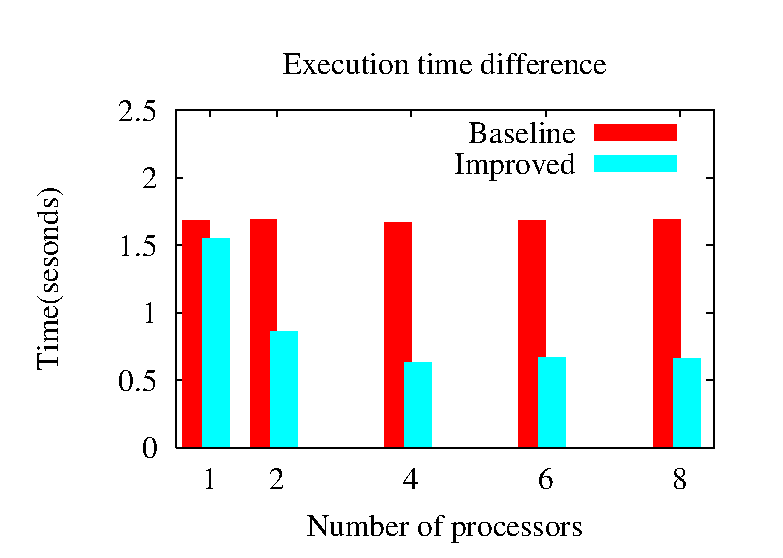
\includegraphics[angle=0, width=0.45\textwidth]{compare.eps}
%    \caption{\footnotesize Performance difference}
%    \label{fig:compare}
%  \end{center}
%\end{figure}

%Figure \ref{fig:compare} show the performance difference of the
%generated code on the POWER4 system. We set \texttt{N} as 100 and
%measured 100 times of the loop nest. In the figure, ``Baseline'' and
%``Improved'' used exactly the same compiler except Algorithm
%\ref{alg:permutepar} is not enabled in the baseline situation. We can
%see that parallel setup overhead completely offset the parallel gains
%in the first case, while the improved version get reasonable speedup
%considering such a little computation cost --- there is only one
%assign statement in the loop nest.


%\subsection{Summary of claims}
%\label{sec:claims}

%We summarize the related claims as following,

%\begin{itemize}
%\item Theorem \ref{theorem:keep}
%\item Algorithm \ref{alg:permutepar} and 
%\item its combination use with Algorithm \ref{alg:permutelocal}
%\end{itemize}

%By fine tuning the heuristics we used in Algorithm
%\ref{alg:permutepar}, we believe we can balance the need for data
%locality and coarse-grained parallelism.

\section{Summary}

Theorem \ref{theorem:keep} provides a simple way to check whether the
loop interchanged is still legal to be parallelized. We can further
use it to develop loop-permutation algorithms.


%%\newpage

\section{Performance data and analysis}
\label{performance}

We measured the EPCC benchmark using various barrier designs to show
the differences in performance overhead. 


Figure \ref{fig:power4performance} shows the barrier overhead for each
kind of implementations on a 32-way POWER4 system with varying numbers
of threads. We used different labels to tag different designs.
\emph{FetchAndAdd} is for the first and the simplest barrier design.
\emph{DistCounter} is used for the barrier with distributed counter.
\emph{DistCounterPad} is used for the barrier with padded distributed
counter. \emph{LocalSensor} is for the barrier using local sensor. And
the last one, \emph{Combined} represents our new barrier scheme, the
barrier with distributed counter combined with local sensor.

\begin{figure*}[!htbp]
  \begin{center}
    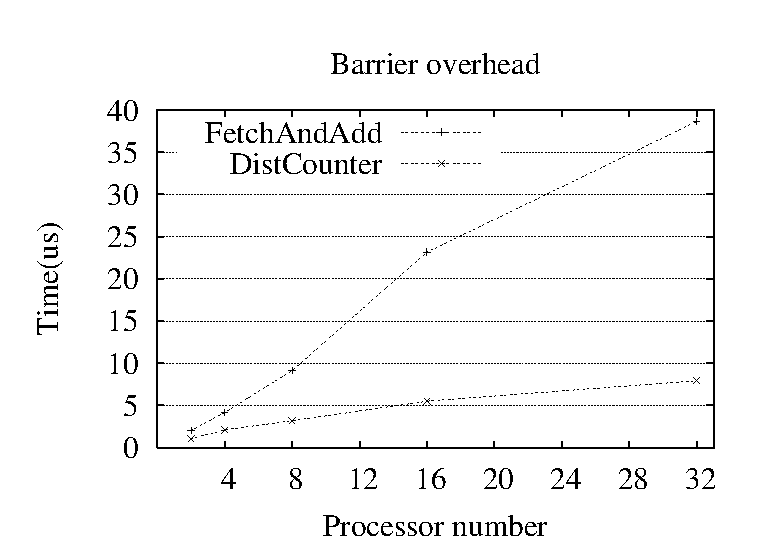
\includegraphics[angle=0, width=0.9\textwidth]{power4performance.eps}
    \caption{POWER4 barrier overhead}
    \label{fig:power4performance}
  \end{center}
\end{figure*}

To further understand the behavior of these barrier designs, we
repeated the tests on a 16-way 375MHz POWER3 system.  Figure
\ref{fig:power3performance} shows the overheads on POWER3.

\begin{figure*}[!htbp]
  \begin{center}
    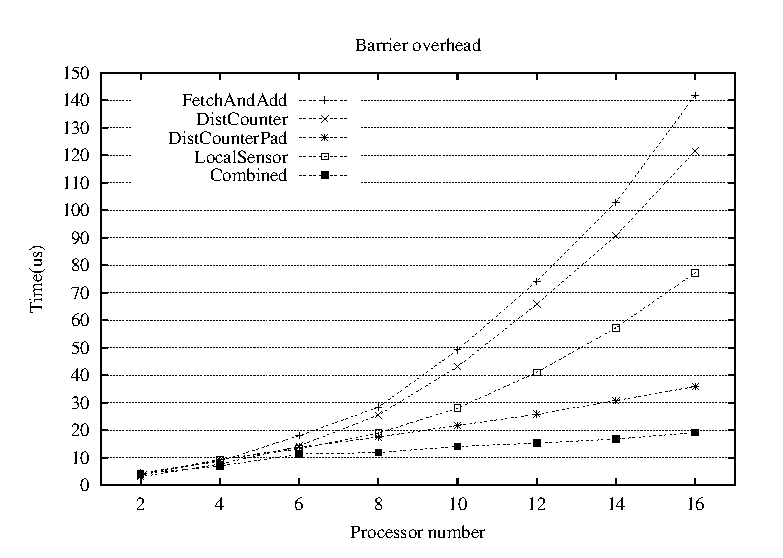
\includegraphics[angle=0, width=0.9\textwidth]{power3performance.eps}
    \caption{POWER3 barrier overhead}
    \label{fig:power3performance}
  \end{center}
\end{figure*}

Although POWER4 and POWER3 have different memory
architectures\cite{Ste98}, one can see that there is little difference
in the relative overhead for different barrier designs. Of course, we
could not compare the scalability of the designs beyond 16 threads on
the POWER3 system so a completely equitable comparison was not
possible.

From the figures we can see that the scalability of the overhead
is not exactly the same, even considering the difference of the clock
speed of the processors --- recall that the POWER4 system we used is
1.1GHz and the POWER3 is 375MHz. The memory system in POWER4 system
certainly gives it extra advantage.

To be able to compare the different implementations, we examine the
performance counters on the more interesting POWER4 system, using
\texttt{pmcount} program available on AIX 5.1. The program will print
out the values of the different performance counters on each
processor, when monitoring a given execution program.

\begin{figure*}[!h]
  \begin{center}
    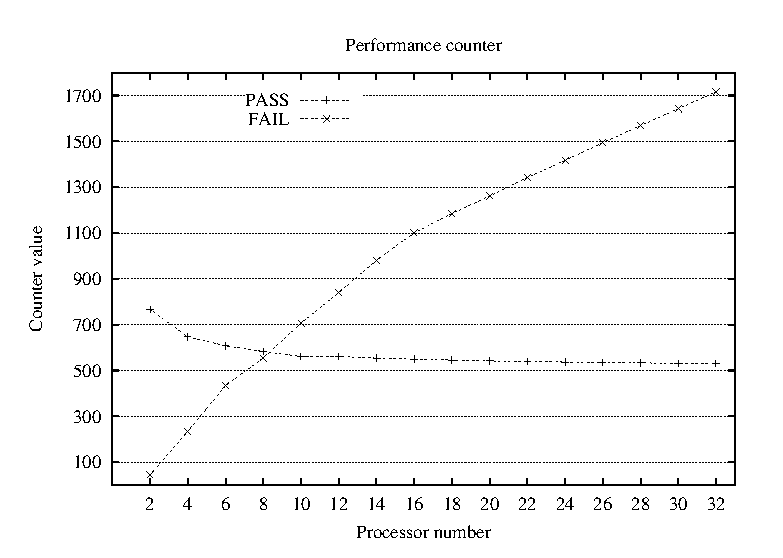
\includegraphics[angle=0, width=0.9\textwidth]{stcx.eps}
    \caption{Store conditional instruction pass and fail}
    \label{fig:stcx}
    \end{center}
\end{figure*}

First we do a simple measurement for the fetch-and-add barrier, using
the exact same setting as we measure overhead previously. We check the
performance counter for store conditional instruction to see the
relationship between contention and the number of processors involved
in a barrier operation. Figure \ref{fig:stcx} shows the average number
of pass and fail for the store conditional instructions on each
processor.

As one can see, while the number of pass remained almost the same(in
theory, it should be identical since we have the same number of
barrier for different number of processors, we consider it is
measurement error here), the number of fail increased sharply as more
processors are added.  That explains why we can not have a scalable
performance for fetch-and-add barrier.

%The barrier implemented with local sensor will has the same problem.

Similarly, we can get the performance counter for cache misses,
representing data traffic. An interesting case here is L2 miss for
distributed counter.

For a POWER4 system, an L2 miss may be served by L2 from another L2 in
the same MCM, L2 in a different MCM, L3 in the same MCM and L3 in a
different MCM. We put them all together as L2 misses. Figure
\ref{fig:lsource} pictures average L2 misses on different processors
for barrier with distributed counter and padded distributed counter.

\begin{figure*}[!h]
  \begin{center}
    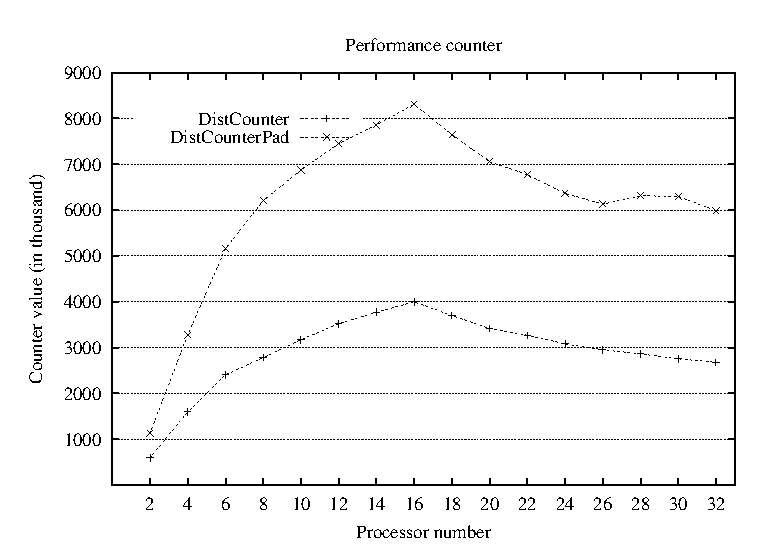
\includegraphics[angle=0, width=0.9\textwidth]{lsource.eps}
    \caption{L2 misses}
    \label{fig:lsource}
    \end{center}
\end{figure*}

To our surprise, there are more cache misses in the barrier with
padded counter, even though it cost less time. We are not sure what
exactly caused this, but we suspect that the cache coherent algorithm
used in hardware cause extra contention when different processors
accessing the same cache line, which out weighs the traffic overhead
caused by L2 misses.

%\begin{verbatim}
%...
%[We are currently working to measure performance 
%counters and analyzing the data.
%The results will be added in the final version of the paper.]
%\end{verbatim}

%Figure \ref{fig:l2misses} shows the mean number of L2 cache misses
%that occurred in all the caches during the execution of 500,000
%barriers as a function of the number of threads participating in the
%barrier. Similarly, Figure \ref{fig:l3misses} shows the L3 cache
%miss behavior (main memory accesses).  Note that, unlike in Figure \ref{fig:l2misses}, the units are not in thousands.

%\begin{figure*}[!htbp]
%  \begin{center}
%    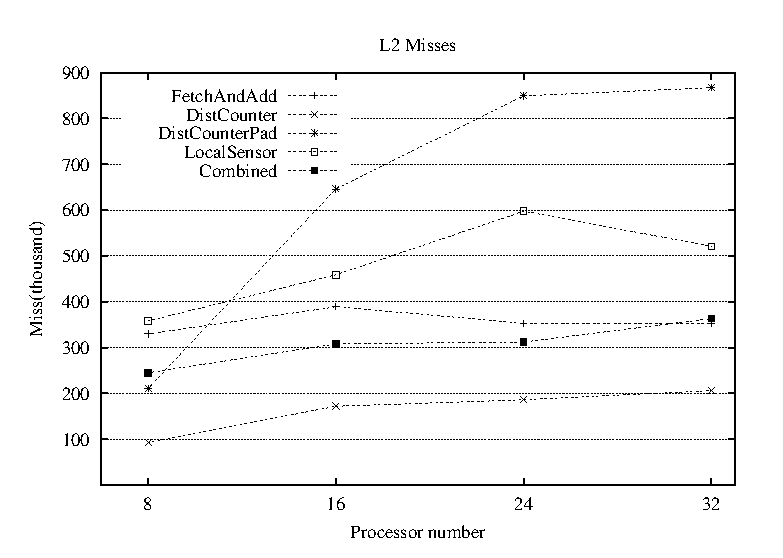
\includegraphics[angle=0, width=0.95\textwidth]{l2miss.eps}
%    \caption{L2 cache misses}
%    \label{fig:l2misses}
%    \end{center}
%\end{figure*}

%\begin{figure*}[!htbp]
%  \begin{center}
%    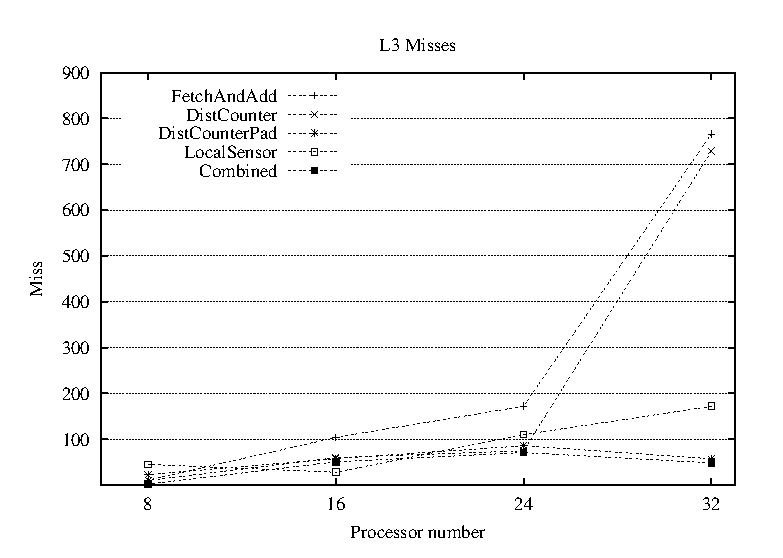
\includegraphics[angle=0, width=0.95\textwidth]{l3miss.eps}
%    \caption{L3 cache misses}
%    \label{fig:l3misses}
%    \end{center}
%\end{figure*}

%We see that the fetch-and-add implementation suffers from a large
%contention problem.  All threads are accessing the same memory location
%at the same time, either signaling arrival or checking if the
%barrier counter is zero. This explains the relatively high number of cache
%misses (including both second and third level) compared to the other
%implementations.

%Each time a given thread reaches the barrier, it has to update the
%counter (and compete for the counter via the fetch-and-add atomic
%operation) and then spin on that counter looking for all changes. This
%will generate a considerable amount of memory traffic as threads will try
%to access the memory position but will need to obtain a valid copy due to
%intervening writes. One
%by one, threads will grab the counter and invalidate all cache lines
%of the other spinning processors.  This will induce all other
%processors to issue a new request for data, forcing a new miss in the cache.
%When the $n^{th}$ thread updates the counter, all spinning threads
%will have their cache line invalidated and will request the line again,
%causing $(n-1)$ misses (1 per cache).

%In total, the first thread that reaches the barrier will fail $(n-1)$
%times due to this effect while the last one will not have misses (but
%will have misses for accessing the counter). This justifies why it has
%the worst L3 behavior, and why it does not scale smoothly.

%The second implementation, DistCounter, mitigates this cache coherence problem to some
%degree. Threads spin in different memory positions (avoiding
%contention) even though the distributed counters share a cache line with some
%other distributed counters.  This barrier implementation also saves overhead
%by avoiding the need for an atomic memory operation.

%We can see that this behavior is greatly reflected in the
%number of L2 cache misses.  The scalability curve has changed from a rather steep line to a
%flatter one. This is mainly due to the fact that the weight of the
%barrier is in the first phase of signaling arrival. The first
%implementation uses fetch-and-add, while the second uses a simple
%store. Nevertheless, false sharing is
%encountered due to the sharing of cache lines among counters.  This explains the L3 cache behavior.

%In contrast, the third implementation, DistCounterPad, is similar to
%DistCounter but tries to eliminate the false sharing problem. Placing
%the whole distributed counter into only one cache line has the
%inconvenience that only one processor can have that line in modified
%state.  The padding tries to enhance the behavior by reducing the
%number of external invalidations.  However, it has a bad L2 cache
%behavior, but as L3 is more important for the overall execution time,
%it is faster than the previous one.

%Each of these techniques addresses the ``entry'' phase of the barrier.  We will see now the effect of optimizing the ``exit'' phase.

%The LocalSensor implementation, which uses a fetch-and-add mechanism,
%is the first one to reduce the overhead in the ``exit'' phase of a
%barrier. Since it does nothing to improve the ``entry'' phase, we get
%better behavior than the first barrier, but not significantly better
%from the DistCounter and DistCounterPad implementations.

%Not surprisingly, the Combined implementation, that benefits from an
%enhanced behavior in both phases, performs better than all the other
%implementations. This is due to the fact that the number of L3 misses
%decreases significantly because of the low degree of communication. Each
%cache line will be accessed only by its corresponding thread and one additional time by the master
%thread.  These cache lines will have no other remote accesses, regardless of
%the number of threads participating in the barrier. That gives us a rather flat line,
%and explains why this implementation is considerably more scalable
%than the previously studied barrier designs.


%%\newpage

\section{Summary and future work}


In this paper, we listed important data structures needed in our
runtime library to support workshares in OpenMP standard, and the
corresponding algorithms to reduce the runtime overhead.

We explained that by carefully choosing the length of the workshare
control block queue, and reusing the queue whenever a barrier
synchronization occurred, we do not need to map control block
structures to memory for each workshare instance.  Also by preparing
the next workshare control block in advance, we do not need a separate
locking phase to initialize a control block, neither do we need to
initialize the whole queue at startup, which saves the parallel
region overhead for most of the real application cases. Although these
are just ``small techniques'', they do have significant impact on
performance benchmarks for runtime libraries.

We also introduced our view on OpenMP workshare, and algorithms to
implement barrier synchronization, which was considered as a special case of the
workshare. All these are commercial available in our XL Fortran and
VisualAge\textregistered\  C/C++ compilers. We are actually further improving the
barrier performance by taking advantage of more accurate cacheline
alignment of our internal data structures.


% how about irregular

%\section{Acknowledgments}

Roch Archambault (from the IBM Toronto Lab) had useful discussions with us;
Raul Silvera and Shimin Cui (from the IBM Toronto Lab) gave us valuable
technical assistance during the integration of the new barrier scheme
to the existing SMP runtime frame work.

\section{Trademarks and copyright}

\textregistered IBM and VisualAge are registered trademarks of
International Business Machines Corporation in the United States,
other countries or both. Other company, product, or service names may
be trademarks or service marks of others.

\noindent
\copyright Copyright International Business Machines Corporation,
2003. All rights reserved.




%--------------------

\bibliographystyle{unsrt}
\bibliography{permutation}

%--------------------

\end{document}

%------------------------------------------------------------------------- 
To do list
%------------------------------------------------------------------------- 

